% === Fig. 3: AQuA first200 exploratory result comparison ===
\begin{figure*}[t]
    \centering
    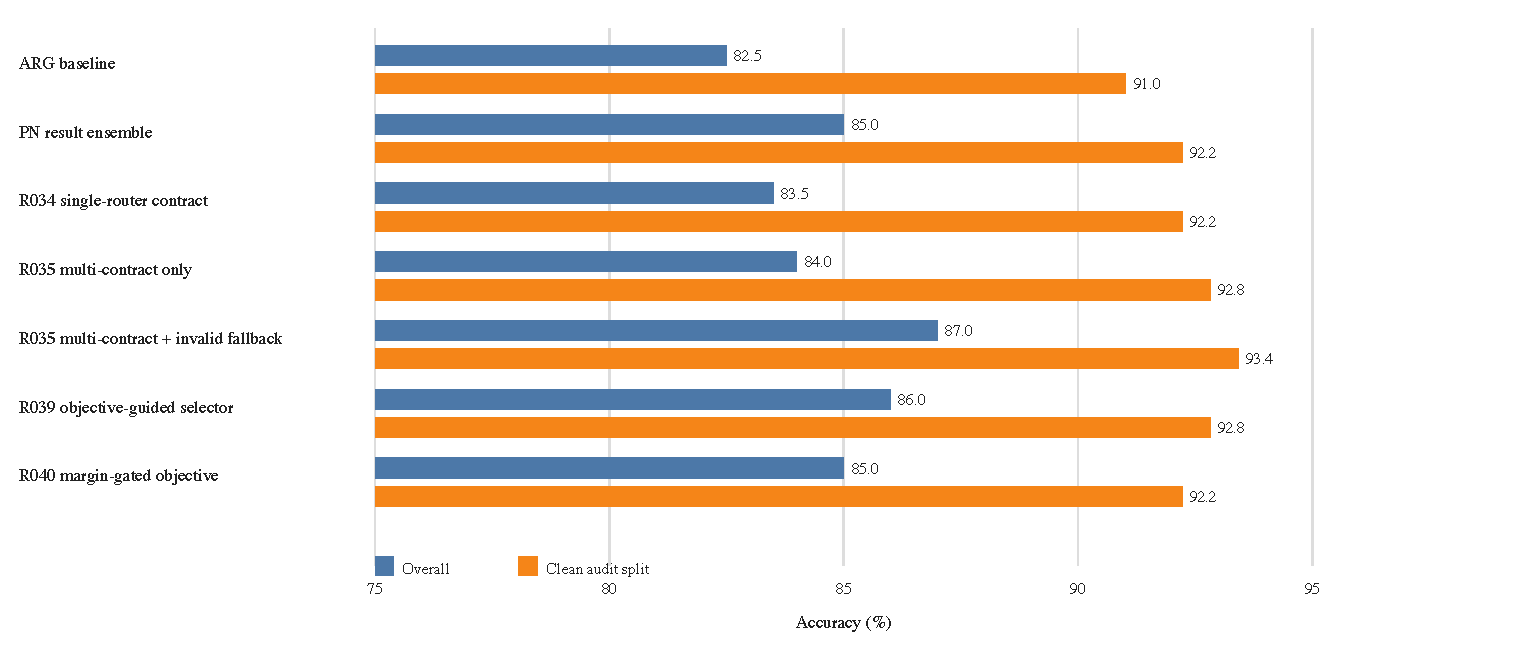
\includegraphics[width=0.95\textwidth]{figures/fig3_aqua_first200_results.pdf}
    \caption{Exploratory AQuA first200 accuracy under the ARG-Designer-compatible setup. The clean split contains 167 audited clean rows. R035 multi-contract only isolates the virtual PromptNode mechanism; R035 full additionally includes invalid-answer fallback.}
    \label{fig:aqua_first200_results}
\end{figure*}

% === Fig. 4: Contract-coverage objective diagnostics ===
\begin{figure}[t]
    \centering
    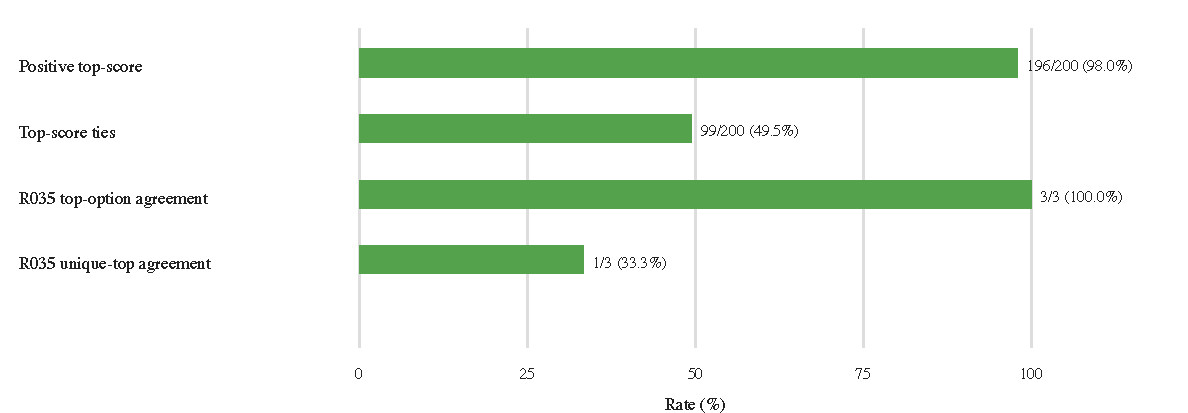
\includegraphics[width=0.48\textwidth]{figures/fig4_contract_coverage.pdf}
    \caption{Label-free contract-coverage objective diagnostics on AQuA first200. The objective covers all three R035 clean-switch options at the top-option level, but ties remain frequent, motivating margin-gated or trained graph selection.}
    \label{fig:contract_coverage}
\end{figure}

% === Table: AQuA first200 main results ===
\begin{table*}[t]
\centering
\caption{AQuA first200 exploratory results under the ARG-Designer-compatible evaluation setup. Clean and noisy/ambiguous splits come from post-hoc option-binding audit; selector decisions do not use audit labels.}
\label{tab:aqua_first200_main_results}
\small
\begin{tabular}{lccccccc}
\toprule
Variant & Overall & Clean & Noisy/Amb. & $\Delta$ & Fix/Harm & Clean F/H & Switches \\
\midrule
ARG baseline & 165/200 & 152/167 & 13/33 & +0 & 0/0 & 0/0 & 0 \\
PN result ensemble & 170/200 & 154/167 & 16/33 & +5 & 9/4 & 3/1 & 22 \\
R034 single-router contract & 167/200 & 154/167 & 13/33 & +2 & 2/0 & 2/0 & 2 \\
R035 multi-contract only & 168/200 & 155/167 & 13/33 & +3 & 3/0 & 3/0 & 3 \\
R035 multi-contract + invalid fallback & 174/200 & 156/167 & 18/33 & +9 & 9/0 & 4/0 & 14 \\
R039 objective-guided selector & 172/200 & 155/167 & 17/33 & +7 & 9/2 & 4/1 & 16 \\
R040 margin-gated objective & 170/200 & 154/167 & 16/33 & +5 & 5/0 & 2/0 & 7 \\
\bottomrule
\end{tabular}

\vspace{0.25em}
\begin{minipage}{0.97\textwidth}
\footnotesize Claim roles: ARG baseline: primary baseline; PN result ensemble: complementarity; harms exist; R034 single-router contract: single-view PN signal; R035 multi-contract only: main mechanism candidate; R035 multi-contract + invalid fallback: full system; fallback separated; R039 objective-guided selector: rejected as main due clean harm; R040 margin-gated objective: safe system candidate.
\end{minipage}
\end{table*}

